\documentclass[11pt]{article}
% !TeX program = pdflatex
% !BIB program = bibtex

% Change "review" to "final" to generate the final (sometimes called camera-ready) version.
% Change to "preprint" to generate a non-anonymous version with page numbers.
\usepackage{acl}

% Standard package includes
\usepackage{times}
\usepackage{latexsym}
\usepackage{amsmath}

% For proper rendering and hyphenation of words containing Latin characters (including in bib files)
\usepackage[T1]{fontenc}
% For Vietnamese characters
% \usepackage[T5]{fontenc}
% See https://www.latex-project.org/help/documentation/encguide.pdf for other character sets

% This assumes your files are encoded as UTF8
\usepackage[utf8]{inputenc}

% This is not strictly necessary, and may be commented out,
% but it will improve the layout of the manuscript,
% and will typically save some space.
\usepackage{microtype}

% This is also not strictly necessary, and may be commented out.
% However, it will improve the aesthetics of text in
% the typewriter font.
% \usepackage{inconsolata}

%Including images in your LaTeX document requires adding
%additional package(s)
\usepackage{graphicx}
\newcommand{\tablefont}{\footnotesize}

% If the title and author information does not fit in the area allocated, uncomment the following
%
%\setlength\titlebox{<dim>}
%
% and set <dim> to something 5cm or larger.

\title{TrustLayer: Verification-Aware Retrieval-Augmented Generation for Reliable Research Assistance}

\author{
  Nikhil Juluri \quad
  Hamsini Pulugurtha \quad
  Ganesh Katta \\
  Department of Computer Science \\
  University of Illinois at Chicago \\
  Chicago, IL, USA \\
  \texttt{\{njulu, hpulu, gkatt\}@uic.edu}
}

\begin{document}
\maketitle
\begin{abstract}
Reliable question answering over local research-paper collections remains difficult because retrieved passages can be noisy, incomplete, or weakly aligned with user intent, and language models may still produce fluent but unsupported claims. We present TrustLayer, a verification-aware Retrieval-Augmented Generation (RAG) framework for reliability-focused research assistance over heterogeneous PDF corpora. TrustLayer separates processing into offline corpus preparation and online inference. Offline, the system performs metadata-aware PDF ingestion, manifest-based cache invalidation, page-level parsing, chunk generation, embedding construction, and vector indexing. Online, it combines dense retrieval from Chroma with BM25 sparse retrieval, merges candidates with reciprocal rank fusion, reranks query--chunk pairs with a cross-encoder, and generates answers using evidence-only prompts.

To improve trustworthiness, TrustLayer adds a multi-signal verification layer that aggregates retrieval confidence, reranker confidence, lexical evidence coverage, semantic evidence similarity, and NLI-based grounding and contradiction scores. A deterministic abstention policy then decides whether to return a grounded answer with evidence metadata or \emph{Insufficient evidence}. The pipeline also preserves intermediate artifacts (manifest, chunk cache, retrieval candidates, and verification outputs) for inspection, reproducibility, and failure analysis.

We evaluate on a cleaned benchmark of 150 questions (132 answerable, 18 unanswerable) over a local corpus of 94 unique research papers. The final system uses 1200/250 chunking, dense/sparse retrieval depths of 50/50, fusion depth 100, and final top-$k=10$. Under strict chunk-level matching, the best BGE-base configuration achieves HitRate@10 = 0.3030, Recall@10 = 0.2955, and PaperHit@10 = 0.4318, outperforming an MPNet ablation under the same setup. Results show a persistent gap between exact chunk recovery and paper-level retrieval, highlighting why verification and abstention are essential for practical research assistants. Overall, TrustLayer demonstrates a reproducible, inspectable architecture for reliability-focused RAG in noisy local environments.
\end{abstract}

\section{Introduction}

Retrieval-Augmented Generation (RAG) improves language model grounding by retrieving external evidence before answer generation. However, RAG systems remain vulnerable to hallucination: a model may produce an answer that is fluent but not supported by the retrieved context, or it may overstate weak evidence as certain. These failures are especially problematic in research-paper assistance, where users need citations, page-level evidence, and clear signals about whether an answer is sufficiently supported.

TrustLayer addresses this problem by treating retrieval, generation, and verification as separate reliability stages. The system first ingests local research papers, creates reusable page and chunk artifacts, retrieves evidence using both semantic and lexical signals, reranks candidate chunks, and only then asks a language model to produce a grounded answer. After generation, TrustLayer computes verification signals and confidence scores. When these signals indicate weak support, the system abstains rather than forcing an answer.

The project is motivated by three practical observations. First, local research-paper corpora are often heterogeneous and noisy, containing PDFs with inconsistent metadata and imperfect text extraction. Second, dense retrieval alone can miss exact terminology, while lexical retrieval alone can miss semantic paraphrases. Third, retrieved evidence does not guarantee that the generated answer is faithful. A trust-aware system therefore needs hybrid retrieval, grounded prompting, post-generation verification, and abstention.

TrustLayer is designed around four reliability goals. First, every answer should be traceable to retrieved evidence chunks. Second, retrieval should combine semantic and lexical matching so that both paraphrased concepts and exact technical terms are represented. Third, generation should be constrained by an explicit evidence-only prompt rather than open-ended model knowledge. Fourth, answers should be rejected when retrieval and verification signals are too weak. These goals make the system closer to a research assistant than a general chatbot: it is allowed to abstain when the available evidence is insufficient.

Unlike a standard RAG demo, TrustLayer emphasizes inspectability. Each intermediate artifact is made explicit: loaded pages are cached, chunking parameters are stored, vector-database configuration is recorded, retrieved chunks retain paper metadata, and evaluation outputs are written as CSV tables. This makes the system easier to audit when a response fails. For example, a low-quality answer can be traced to the original PDF text extraction, the generated chunk, the dense or sparse retrieval stage, the reranker score, or the verification gate. This practical transparency is important for research settings, where users may need to understand not only the final answer but also the retrieval path that produced it.

This paper makes the following contributions:

\begin{itemize}
    \item We present a complete local RAG architecture for research-paper corpora, including PDF ingestion, chunking, vector storage, hybrid retrieval, reranking, generation, verification, and abstention.
    \item We implement hybrid retrieval with dense Chroma search, BM25 sparse retrieval, reciprocal rank fusion, and cross-encoder reranking.
    \item We introduce a verification layer that combines retrieval confidence, reranker confidence, evidence similarity, evidence coverage, NLI entailment, contradiction checks, and combined confidence.
    \item We construct a cleaned 150-question evaluation set with answerable and unanswerable questions and report retrieval, paper-level, and verification metrics.
    \item We provide report-generation utilities that produce reproducible tables and figures from evaluation CSV outputs.
\end{itemize}

\section{Related Work}

\paragraph{Retrieval-Augmented Generation.}
RAG systems retrieve external documents or passages and condition generation on the retrieved context \citep{lewis2020rag}. This design improves factual grounding relative to closed-book generation, but retrieved passages can still be irrelevant, incomplete, or misused by the generator. TrustLayer follows the RAG paradigm but adds verification and abstention after generation.

\paragraph{Hybrid Retrieval.}
Dense retrievers represent queries and documents in embedding space, while sparse methods such as BM25 rely on lexical overlap \citep{robertson2009bm25}. Dense passage retrieval demonstrated the effectiveness of learned passage representations for open-domain question answering \citep{karpukhin2020dpr}, while sentence embedding models made semantic similarity search practical at scale \citep{reimers2019sbert}. Hybrid systems combine these complementary signals, often improving robustness across paraphrased and keyword-heavy queries. TrustLayer uses dense Chroma retrieval together with BM25 and reciprocal rank fusion \citep{cormack2009rrf}.

\paragraph{Reranking.}
Cross-encoder rerankers score query--passage pairs more directly than independent embeddings. They are commonly used after an efficient first-stage retriever to improve the ordering of a smaller candidate set \citep{nogueira2019passage}. TrustLayer reranks fused candidates with \texttt{cross-encoder/ms-marco-MiniLM-L-6-v2}.

\paragraph{Hallucination Detection and Verification.}
Hallucination detection methods estimate whether generated text is supported by source evidence \citep{ji2023survey}. NLI-based verification is a common approach for checking entailment or contradiction between evidence and claims \citep{thorne2018fever}. TrustLayer combines NLI signals with retrieval and semantic similarity scores rather than relying on a single verifier.

\paragraph{Confidence Calibration.}
Confidence calibration aims to align system scores with expected correctness \citep{guo2017calibration}. In RAG, calibrated confidence can support abstention when retrieved evidence is weak. TrustLayer computes a combined confidence score from retrieval, reranking, evidence coverage, semantic similarity, and grounding signals, and uses this score in a verification gate.

\paragraph{Abstention in Question Answering.}
Selective prediction and abstention mechanisms allow a system to avoid answering when confidence is low. For evidence-grounded QA, abstention is useful because an incorrect answer may be more harmful than no answer. TrustLayer uses a deterministic abstention rule based on retrieval, semantic, lexical, and NLI-derived verification signals, rather than relying only on the language model's self-reported uncertainty.

\section{Problem Statement}

Given a user question over a local corpus of research-paper PDFs, the goal is to return either (1) an evidence-grounded answer supported by retrieved chunks with source metadata or (2) an abstention response (\emph{Insufficient evidence}) when support is inadequate. Formally, for question $q$ and corpus $\mathcal{D}$, the system must retrieve a ranked set of candidate chunks $E_k \subset \mathcal{D}$, generate answer $a$, and compute verification signals $v$. The system should maximize evidence localization quality and paper-level retrieval quality while minimizing unsupported answers.

This problem is challenging because local PDF corpora are noisy, relevant evidence can be distributed across multiple chunks, and fluent generation may still be ungrounded. Therefore, the project targets three concrete objectives: (1) robust retrieval under lexical and semantic variation, (2) generation constrained to retrieved evidence, and (3) explicit verification and abstention when confidence is low.

\section{Methodology}

Figure~\ref{fig:pipeline} summarizes the TrustLayer pipeline. The system has an offline component for corpus preparation and an online component for question answering, verification, and abstention.

\begin{figure*}[t]
\centering
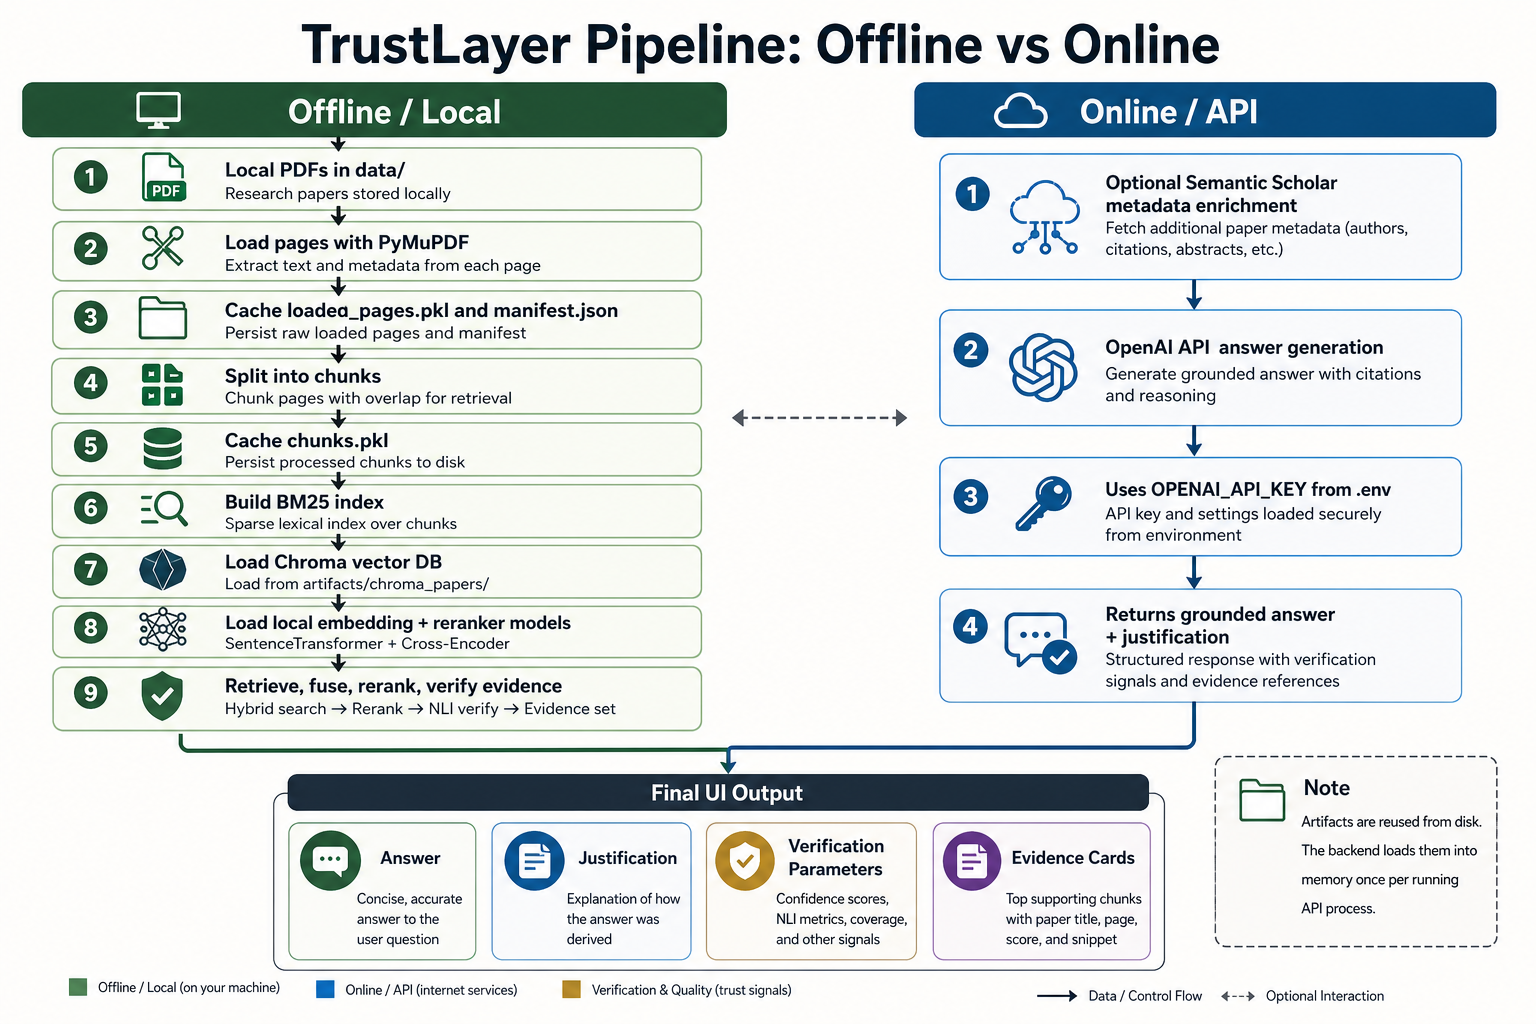
\includegraphics[width=\textwidth]{figures/trustlayer-pipeline-offline-online.png}
\caption{TrustLayer system pipeline architecture with offline and online components.}
\label{fig:pipeline}
\end{figure*}

\subsection{Document Ingestion and Text Parsing}

TrustLayer reads local PDF files from the \texttt{data/} directory. The loader recursively scans domain-specific folders, loads pages with \texttt{PyMuPDFLoader}, and stores each page as a LangChain document. The loader records page number, total pages, filename, relative path, domain, and source path. It skips empty or near-empty pages using a configurable minimum word threshold.

The metadata layer resolves paper titles and authors through a priority order: cached metadata, filename fallback, first-page heuristic extraction, and optional Semantic Scholar enrichment. This design is necessary because embedded PDF metadata is often missing, generic, or corrupted.

The loader also builds a manifest over PDF relative paths, modification times, and file sizes. If the manifest changes, the page-level document cache is invalidated and rebuilt. This prevents stale retrieval artifacts when the local corpus changes. Metadata is stored at the page level and later propagated to chunks, enabling evidence displays with title, filename, page number, and chunk identifier.

\subsection{Chunk Generation}

After page loading, TrustLayer splits documents with a recursive character splitter. The final experimental setup used 1200-character chunks with 250-character overlap. Chunk metadata includes the originating document identifier, page identifier, global chunk index, and stable chunk identifier. Chunk artifacts are cached in \texttt{artifacts/chunks.pkl}; a separate chunk configuration file triggers rebuilding when the chunk size or overlap changes.

The 1200/250 chunking setting was selected after preliminary experiments with smaller chunks. Research papers often express methods, limitations, and experimental findings across multiple sentences. Larger chunks preserve more local context for reranking and generation, while overlap reduces the chance that a relevant statement is split across two retrieval units. The trade-off is that larger chunks produce fewer but longer evidence candidates, which may reduce exact chunk-level recall in some cases.

\subsection{Embedding Generation and Vector Storage}

Embeddings are generated through the Hugging Face embedding wrapper with normalized vectors. The final retrieval experiment used \texttt{BAAI/bge-base-en-v1.5}; an MPNet configuration using \texttt{sentence-transformers/all-mpnet-base-v2} was also evaluated as an ablation. TrustLayer stores vectors in Chroma at \texttt{artifacts/chroma\_papers/}. The Chroma collection metadata specifies cosine HNSW search through \texttt{\{"hnsw:space": "cosine"\}}; HNSW is a graph-based approximate nearest-neighbor method designed for efficient vector search \citep{malkov2020hnsw}.

\subsection{Hybrid Retrieval}

Given a user query, the retrieval module performs dense retrieval from Chroma and sparse retrieval with BM25. BM25 is built in memory over the cached chunks at runtime. Dense and sparse candidates are merged with reciprocal rank fusion. In the final evaluation, TrustLayer used dense top-$k=50$, sparse top-$k=50$, fusion top-$k=100$, and final top-$k=10$.

Reciprocal rank fusion assigns each candidate a score based on its rank in each retrieval list. A chunk that appears in both dense and sparse retrieval receives accumulated support, while chunks found by only one retriever can still be retained. This is useful for research corpora because some queries contain exact method names or datasets, while others use more conceptual paraphrases.

\subsection{Reranking}

Fused candidates are reranked with \texttt{cross-encoder/ms-marco-MiniLM-L-6-v2}. The reranker scores each query--chunk pair, and the system keeps the highest-scoring final evidence chunks. Reranker scores are converted through a sigmoid function and combined into a retrieval confidence score using the top result and the average of the top three results.

\subsection{Grounded LLM Generation}

The generation prompt instructs the language model to use only retrieved evidence and to answer exactly \emph{Insufficient evidence} when support is inadequate. The OpenAI generation module uses \texttt{gpt-4o-mini} with temperature 0 and a function-calling schema containing an answer and evidence-based justification. The context passed to the generator includes title, authors, filename, page number, chunk identifier, and chunk content for each evidence item.

The prompt explicitly forbids outside knowledge. This is important because many questions refer to well-known papers; an unconstrained model could answer from pretraining rather than from retrieved evidence. TrustLayer instead treats retrieved chunks as the only valid source of information. The generated response is normalized into an answer and justification before verification.

The implementation uses structured tool output from the OpenAI API so that generated responses contain a concise answer and a short justification. This reduces parsing ambiguity compared with free-form text. If the model returns exactly \emph{Insufficient evidence}, TrustLayer preserves the abstention rather than attempting to force a justification. This behavior is central to the system's reliability objective: a successful run is not necessarily one that answers every question, but one that distinguishes supported answers from unsupported ones.

\subsection{Verification and Calibration}

TrustLayer verifies generated answers using multiple signals. Evidence similarity is computed between the generated answer and retrieved chunks using normalized sentence embeddings. Evidence coverage measures lexical overlap between answer words and retrieved context words. NLI verification uses \path{MoritzLaurer/deberta-v3-base-mnli-fever-anli} to estimate entailment and contradiction between evidence and answer.

The system computes a grounding score from maximum and top-three entailment values. It also computes a combined confidence score:

\begin{equation}
\begin{split}
C = &0.25 C_r + 0.20 C_{rr} + 0.20 C_c \\
    &+ 0.15 C_s + 0.20 C_g ,
\end{split}
\end{equation}

where $C_r$ is retrieval confidence, $C_{rr}$ is reranker confidence, $C_c$ is evidence coverage, $C_s$ is evidence similarity, and $C_g$ is the grounding score.

\subsection{Abstention Mechanism}

TrustLayer uses verification gates to decide whether an answer is sufficiently supported. The strict pass requires retrieval confidence and reranker confidence of at least 0.35, evidence similarity of at least 0.30, grounding score of at least 0.45, and contradiction below 0.40. A secondary evidence-backed fallback allows high-confidence answers when retrieval, reranking, similarity, coverage, and combined confidence are strong and contradiction remains below 0.50. If neither gate passes, the system abstains and returns \emph{Insufficient evidence}.

\begin{table}[t]
\centering
\tablefont
\setlength{\tabcolsep}{3pt}
\begin{tabular}{p{0.40\columnwidth}p{0.50\columnwidth}}
\hline
\textbf{Verification signal} & \textbf{Threshold / role} \\
\hline
Retrieval confidence & $\geq 0.35$ strict pass \\
Reranker confidence & $\geq 0.35$ strict pass \\
Evidence similarity & $\geq 0.30$ strict pass \\
Grounding score & $\geq 0.45$ strict pass \\
Contradiction & $< 0.40$ strict pass \\
Combined confidence & used in fallback gate \\
\hline
\end{tabular}
\caption{Verification gate signals used by TrustLayer. Thresholds are manually configured from the implemented pipeline.}
\label{tab:thresholds}
\end{table}

\subsection{User Interfaces and Evidence Display}

TrustLayer includes both a Streamlit interface and a React/FastAPI interface. The Streamlit interface exposes tabs for overview, verification, evidence, manual evaluation, and generator context. The React path uses a lightweight router that adjusts retrieval settings based on question type, such as definition, comparison, citation-focused, or mechanism-oriented queries. In both interfaces, retrieved evidence is displayed with metadata so that a user can inspect the supporting chunks rather than only viewing a final answer.

\section{Experiments}

\subsection{Corpus and Evaluation Set}

The final corpus contained 94 unique research papers from 95 PDF files. The papers were stored locally under \texttt{data/} and grouped by domain. The final evaluation set contained 150 generated questions, including 132 answerable questions and 18 unanswerable questions. The question-generation script filtered vague or generic questions, yielding zero vague/generic questions in the final set.

The project data and generated artifacts are included in the project submission package and repository paths \texttt{data/} and \texttt{artifacts/} (PDF corpus metadata, evaluation question CSV files, and report CSV outputs). This satisfies reproducibility requirements for the submitted system configuration.

The questions covered factual, conceptual, methodology, comparison, limitation, multihop, and unanswerable categories. Table~\ref{tab:question-dist} shows the final distribution.

\begin{table}[t]
\centering
\tablefont
\setlength{\tabcolsep}{4pt}
\begin{tabular}{lrr}
\hline
\textbf{Category} & \textbf{Questions} & \textbf{Share} \\
\hline
comparison & 22 & 0.1467 \\
conceptual & 25 & 0.1667 \\
factual & 19 & 0.1267 \\
limitation & 25 & 0.1667 \\
methodology & 22 & 0.1467 \\
multihop & 19 & 0.1267 \\
unanswerable & 18 & 0.1200 \\
\hline
\end{tabular}
\caption{Question distribution in the final cleaned evaluation set.}
\label{tab:question-dist}
\end{table}

\subsection{System Configuration}

The final retrieval configuration used 1200-character chunks, 250-character overlap, BGE-base embeddings, Chroma HNSW cosine vector search, BM25 sparse retrieval, reciprocal rank fusion, and cross-encoder reranking. Metrics were computed at $K \in \{1,3,5,10\}$. Retrieval metrics include Precision@K, Recall@K, HitRate@K, MRR@K, nDCG@K, and PaperHit@K. PaperHit@K measures whether the correct source paper appears among the top-$K$ retrieved chunks, even if the exact annotated chunk is not retrieved.

\begin{table}[t]
\centering
\tablefont
\setlength{\tabcolsep}{3pt}
\begin{tabular}{p{0.34\columnwidth}p{0.56\columnwidth}}
\hline
\textbf{Component} & \textbf{Configuration} \\
\hline
Corpus & 94 papers / 95 PDFs \\
Chunk size / overlap & 1200 / 250 characters \\
Dense embedding & BAAI/bge-base-en-v1.5 \\
Vector DB & Chroma, HNSW cosine \\
Sparse retrieval & BM25 \\
Fusion & Reciprocal rank fusion \\
Reranker & ms-marco-MiniLM-L-6-v2 \\
Dense / sparse $k$ & 50 / 50 \\
Fusion / final $k$ & 100 / 10 \\
Generator & gpt-4o-mini, temperature 0 \\
\hline
\end{tabular}
\caption{Final TrustLayer experimental configuration.}
\label{tab:config}
\end{table}

\subsection{Evaluation Metrics}

Precision@K measures the fraction of retrieved top-$K$ chunks that match annotated evidence chunks. Recall@K measures how many annotated evidence chunks are retrieved. HitRate@K indicates whether at least one annotated evidence chunk appears in the top-$K$ results. MRR@K rewards systems that rank the first relevant chunk earlier. nDCG@K measures ranking quality with position discounting. PaperHit@K is a looser metric that counts whether the correct source paper appears in the top-$K$ retrieved chunks. This distinction is important because strict chunk-level labels can undercount cases where a neighboring chunk or another chunk from the same paper contains useful evidence.

The evaluation questions were generated from sampled chunks and then filtered to remove vague references such as ``the paper,'' ``this work,'' or ``the method'' unless the question contained a clear technical anchor. Each answerable question includes a ground-truth answer and one or two source chunk identifiers. Multihop questions require exactly two source chunks, while unanswerable questions are plausible but intentionally unsupported by the sampled evidence. This construction allows the benchmark to test both evidence retrieval and abstention-oriented behavior. The final report artifacts also include question distribution, category-wise retrieval, embedding ablation, and verification summaries, enabling reproducible comparison across retrieval settings.

\section{Results}

\subsection{Retrieval Performance}

Table~\ref{tab:retrieval} reports final BGE-base retrieval performance. Under strict chunk-level matching, HitRate@10 was 0.3030 and Recall@10 was 0.2955. PaperHit@10 was 0.4318, indicating that the system retrieved the correct source paper more often than the exact annotated evidence chunk.

\begin{table}[t]
\centering
\tablefont
\setlength{\tabcolsep}{3pt}
\begin{tabular}{rrrrrr}
\hline
\textbf{K} & \textbf{Prec.} & \textbf{Rec.} & \textbf{Hit} & \textbf{MRR} & \textbf{nDCG} \\
\hline
1 & 0.1364 & 0.1288 & 0.1364 & 0.1364 & 0.1364 \\
3 & 0.0783 & 0.2235 & 0.2348 & 0.1755 & 0.1829 \\
5 & 0.0561 & 0.2576 & 0.2652 & 0.1827 & 0.1981 \\
10 & 0.0326 & 0.2955 & 0.3030 & 0.1874 & 0.2105 \\
\hline
\end{tabular}
\caption{Final strict chunk-level retrieval performance using BGE-base embeddings. PaperHit@K is reported separately in the text: 0.3485, 0.4015, 0.4091, and 0.4318 for K=1, 3, 5, and 10.}
\label{tab:retrieval}
\end{table}

\subsection{Verification Metrics}

Table~\ref{tab:verification} summarizes the mean verification scores for the BGE-base configuration. These scores provide a trust layer beyond retrieval, estimating whether generated answers are supported by retrieved evidence.

\begin{table}[t]
\centering
\tablefont
\setlength{\tabcolsep}{3pt}
\begin{tabular}{p{0.68\columnwidth}r}
\hline
\textbf{Verification Parameter} & \textbf{Mean} \\
\hline
Retrieval Confidence & 0.4191 \\
Reranker Confidence & 0.4328 \\
Evidence Similarity & 0.2889 \\
Grounding Score & 0.3295 \\
Evidence Coverage & 0.3636 \\
Combined Confidence & 0.3733 \\
NLI Max Entailment & 0.3667 \\
NLI Max Contradiction & 0.2130 \\
\hline
\end{tabular}
\caption{Mean verification and calibration signals for the final BGE-base TrustLayer configuration.}
\label{tab:verification}
\end{table}

\subsection{Embedding Ablation}

Table~\ref{tab:ablation} compares MPNet and BGE-base under the same final chunking and evaluation setup. BGE-base performed slightly better across all reported @10 retrieval metrics.

\begin{table}[t]
\centering
\tablefont
\setlength{\tabcolsep}{2pt}
\resizebox{\columnwidth}{!}{%
\begin{tabular}{p{0.28\columnwidth}rrrr}
\hline
\textbf{Setup} & \textbf{Hit@10} & \textbf{Rec.@10} & \textbf{MRR@10} & \textbf{PaperHit@10} \\
\hline
MPNet + 1200/250 & 0.2879 & 0.2765 & 0.1839 & 0.3939 \\
BGE-base + 1200/250 & 0.3030 & 0.2955 & 0.1874 & 0.4318 \\
\hline
\end{tabular}
}
\caption{Embedding ablation on the final cleaned evaluation set.}
\label{tab:ablation}
\end{table}

\subsection{Category-Level Observations}

Factual questions achieved the strongest category-level strict retrieval result, with HitRate@10 of 0.4211 and PaperHit@10 of 0.5263. Limitation and multihop questions were harder: limitation questions reached HitRate@10 of 0.2400, while multihop questions reached HitRate@10 of 0.2105. This pattern is expected because limitations are often stated diffusely and multihop questions require evidence from multiple chunks.

\begin{table}[t]
\centering
\tablefont
\setlength{\tabcolsep}{3pt}
\resizebox{\columnwidth}{!}{%
\begin{tabular}{lrrr}
\hline
\textbf{Category} & \textbf{Hit@10} & \textbf{Rec.@10} & \textbf{PaperHit@10} \\
\hline
comparison & 0.3182 & 0.2955 & 0.4545 \\
conceptual & 0.3200 & 0.3200 & 0.4800 \\
factual & 0.4211 & 0.4211 & 0.5263 \\
limitation & 0.2400 & 0.2400 & 0.4000 \\
methodology & 0.3182 & 0.3182 & 0.4091 \\
multihop & 0.2105 & 0.1842 & 0.3158 \\
\hline
\end{tabular}
}
\caption{Category-wise retrieval performance at K=10 for the final BGE-base configuration.}
\label{tab:category}
\end{table}

\subsection{Discussion}

The final results show that TrustLayer retrieves the exact annotated evidence chunk for approximately 30\% of answerable questions within the top ten chunks, while retrieving the correct paper for approximately 43\% of questions. The gap between HitRate@10 and PaperHit@10 indicates that the system often identifies the relevant paper but does not always localize the exact annotated chunk. This is a common challenge for long-document RAG over research papers, where related evidence may appear in adjacent or semantically overlapping chunks.

The embedding ablation shows that BGE-base slightly outperformed MPNet under the same final chunking and retrieval settings. The difference is modest, but consistent across HitRate@10, Recall@10, nDCG@10, and PaperHit@10. Verification scores were moderate rather than high, suggesting that retrieval and grounding remain challenging under strict evidence matching. However, these scores are useful because they provide interpretable signals for abstention rather than treating all generated answers as equally reliable.

The results also show the value of reporting both chunk-level and paper-level metrics. Chunk-level matching is strict and evaluates exact evidence localization, while PaperHit measures whether the broader source document is recovered. TrustLayer's higher PaperHit values indicate that retrieval sometimes reaches the correct paper but not the exact annotated chunk. In a user-facing research assistant, this behavior is still useful because reranking, generation, and evidence inspection may surface related context, but it also motivates future work on local evidence refinement after paper-level retrieval succeeds.

\section{Limitations}

TrustLayer was evaluated on a local corpus of 94 unique papers, which limits claims about generalization to larger or more diverse collections. Some PDFs contained noisy or corrupted extracted text, which can reduce retrieval quality, sparse matching, question generation quality, and evidence localization. The evaluation uses strict chunk-level matching; a neighboring chunk or another chunk from the correct paper may contain useful evidence but still be counted as incorrect. The verification layer adds computational overhead because it requires additional embedding and NLI model inference. The system also depends on external model behavior, including OpenAI generation, Hugging Face embedding models, a cross-encoder reranker, and an NLI model. Finally, the confidence thresholds were manually configured rather than learned from a large calibration set.

Another limitation is that the evaluation questions were generated from the corpus using an LLM and then filtered heuristically. This makes the benchmark useful for repeatable system testing, but it is not equivalent to a manually authored expert benchmark. Future evaluations should include human validation of question quality, evidence labels, and answer correctness.

\section{Future Work}

Future work should improve both retrieval quality and evaluation fidelity. One direction is OCR and extraction cleanup for noisy PDFs, especially papers whose text is corrupted by mathematical notation, ligatures, multi-column layout, or scanned content. Better PDF normalization would improve both dense embeddings and BM25 token matching. A second direction is neighbor-aware evidence matching: if the system retrieves a chunk adjacent to the annotated source chunk, the evaluation could distinguish near misses from fully incorrect retrieval. This would better reflect the behavior of long-document RAG systems, where useful evidence often spans chunk boundaries.

Another direction is learned calibration. TrustLayer currently uses manually selected thresholds for retrieval confidence, reranker confidence, semantic similarity, grounding, contradiction, and combined confidence. A larger validation set could support data-driven calibration, threshold tuning, and reliability diagrams. The system could also evaluate stronger rerankers, larger retrieval-focused embedding models, and domain-specific query expansion. Finally, future user studies could measure whether the verification table, evidence display, and abstention behavior improve user trust and reduce unsupported answer acceptance.

\section{Team Work Division and Overall Experience}

\noindent\textbf{Nikhil Juluri} led end-to-end pipeline integration, including corpus ingestion/caching, chunking, hybrid retrieval orchestration, evaluation scripts, and report artifact generation.

\vspace{0.35em}
\noindent\textbf{Hamsini Pulugurtha} focused on verification and confidence design, including evidence similarity and coverage features, NLI-based grounding/contradiction checks, and abstention threshold analysis.

\vspace{0.35em}
\noindent\textbf{Ganesh Katta} focused on user-facing system components and analysis support, including Streamlit/React interface integration, evidence display flows, and experiment/result validation.

\vspace{0.35em}
\noindent As a team, we found that building a reliable research assistant required stronger engineering around data quality and evaluation than expected. The main practical lesson was that transparent verification and abstention behavior are as important as retrieval quality for user trust.

\section{Conclusion}

TrustLayer is a verification-aware RAG framework for local research-paper question answering. It combines metadata-aware PDF ingestion, chunking, dense and sparse retrieval, reciprocal rank fusion, reranking, grounded generation, multi-signal verification, confidence calibration, and abstention. The final BGE-base configuration achieved the strongest retrieval performance in the local evaluation and produced interpretable verification metrics. Overall, the system shows how RAG pipelines can be made more reliable by combining evidence retrieval with explicit post-generation verification and abstention.

\bibliography{custom}
\end{document}
